\section{Information bottleneck: Triplet comparisons versus Quadruple comparisons}

In this section, we will discuss the consistency up to which triplet and quadruple comparisons specify a given distance function. Consider a distance function $d$ on an arbitrary sample space $\cX$ (can be any well-defined object). First, we define quadruple comparison in the following.

\paragraph{Quadruple comparisons:} In Section 2, we defined the concept of oblivious teaching of a metric \( d \in \mathcal{M} \) using triplet comparisons (see \eqnref{eq: sol}). An extension to triplet comparisons is the notion of quadruple comparisons. For any given points \( v_1, v_2, v_3, v_4 \), a comparison of the form \( (v_1, v_2, v_3, v_4)_q \) denotes
\begin{align*}
 (v_1, v_2, v_3, v_4)_q
    = \begin{cases}
        = & \textnormal{if } d(v_1, v_2) = d(v_3, v_4)\\
        < & \textnormal{if } d(v_1, v_2) < d(v_3, v_4)\\
        > & \textnormal{if } d(v_1, v_2) > d(v_3, v_4)
    \end{cases}
\end{align*}
If \( v_1 = v_3 \), then the quadruple comparison reduces to a triplet comparison, thus generalizing the notion of triplet comparisons. It is straightforward that quadruple comparisons are at least as informative as triplet comparisons. In the following, we will demonstrate that they are strictly more informative for oblivious teaching of a graph distance function.

We want to understand whether two comparisons of interest, triplet, and quadruples, can fully specify a distance function $d$ up to monotonic transformation $f$ which is defined as follows:
%\sanjoy{I think it would be better to avoid using capital script for the transformation since we have otherwise been using it for classes. Maybe just $f$ instead of $\cF$?}

\begin{definition}\label{def: monotonic}
    Define a scalar transformation $f: \reals \to \reals$. We call $f$ to be strictly monotonically increasing if for all scalars $u < v$ we have $f(u) < f(v)$.

\end{definition}
%\sanjoy{We will actually need it to be strictly monotonic.}

Now, let $w: E \to \reals_{+}$ be the weights or distances between the nodes in $\cX_N$ as assigned by $d$.
We say a learner learns a distance function $d$ upto monotonic transformation if for all such $f$ and for any $w_i,w_j \in w$ $f(w'_{i}) \le f(w'_j)$ if $w_i \le w_j$ where $(d',w')$ is the learned distance function.
Note that a (strict) monotonic transformation on a real line is invertible. Thus, if a distance function $d$ is learnt up to monotonic transformation, then there exists $f$ such that
\begin{align*}
    f^{-1}(w') = w
\end{align*}
We are interested in understanding the information bottleneck of triplet versus quadruple comparisons in specifying a distance function. We study this as an equivalence property induced by distance specification up to monotonic transformation as defined in \defref{def: monotonic}.
\begin{definition}
    Consider two distance functions $d,d'$ on a sample space $\cX$. We say $d$ and $d'$ are ordinally equivalent, if they are equivalent up to strictly monotonic transformation, i.e.
    \begin{align*}
        \exists \textnormal{ a mono. trans. } f,\, s.t.\,\, \forall x,y \in \cX,  \quad d'(x,y) = f (d(x,y)).
    \end{align*}
\end{definition}

We are interested in understanding if triplet comparisons can specify $d$ up to ordinal equivalence. The answer is negative, i.e. triplet comparisons alone can't specify $d$ up to ordinal equivalence. The counterexample is a simple path distance function of length 3 as follows:

\begin{lemma}
    For a path metric $d$ on four points $a,b,c,d$ such that $d(a,b) = 3$, $d(b,c) = 4$ and $d(c,d)= 2$. Triplet comparisons can't specify $d$ up to ordinal equivalence.
\end{lemma}
\begin{figure}[ht!]
    \centering
    \begin{subfigure}[b]{0.8\textwidth}
        \centering
        \begin{tikzpicture}
            % First diagram
            \node (a) at (0,0) {a};
            \node (b) at (3,0) {b};
            \node (c) at (7,0) {c};
            \node (d) at (9,0) {d};

            \draw (a) -- (b) node[midway, above] {3};
            \draw (b) -- (c) node[midway, above] {4};
            \draw (c) -- (d) node[midway, above] {2};
        \end{tikzpicture}
        \caption{Correct metric $d$}
        \label{fig:correct_metric}
    \end{subfigure}
    
    \vspace{1cm} % Adjust the space between the diagrams as needed

    \begin{subfigure}[b]{0.8\textwidth}
        \centering
        \begin{tikzpicture}
            % Second diagram
            \node (a2) at (0,0) {a};
            \node (b2) at (2,0) {b};
            \node (c2) at (6,0) {c};
            \node (d2) at (9,0) {d};

            \draw (a2) -- (b2) node[midway, above] {2};
            \draw (b2) -- (c2) node[midway, above] {4};
            \draw (c2) -- (d2) node[midway, above] {3};
        \end{tikzpicture}
        \caption{Possible triplet comparisons induced metric}
        \label{fig:possible_metric}
    \end{subfigure}
    
\end{figure}
\begin{proof}
 Note that the path metric specified in \figref{fig:possible_metric}, denoted as $d'$ satisfies all possible triplet comparisons on the metric $d$ as shown in \figref{fig:correct_metric}:
 \begin{align*}
     (a,b,c), (a,b,d), (a,c,d), (b,a,c),(b,a,d), (b,c,d),\ldots, (d,c,b), (d,c,a), (d,b,a)
 \end{align*}
 But $d'(a,b) < d'(c,d)$ whereas $d(a,b) > d(c,d)$.
\end{proof}

This issue arises because triplet comparisons can't specify the ordering of the distances $d(a,b)$ and $d(c,d)$. Essentially, it only specifies the ordering with respect to a center (node) not when we compare distances without fixing a center. We can resolve this issue with \tt{quadruples}.

\begin{lemma}
    Consider $\cX$ to be an underlying sample space, and $d: \cX \to \cX \to \reals$ be a target distance function. Then, quadruplets specify $d$ up to ordinal equivalence.%, i.e. learner finds a distance function $d': \cX \times \cX \to \reals$ such that 
    %\begin{align*}
    %    \exists \textnormal{ a mono. trans. } f,\, s.t.\,\, \forall x,y \in \cX,  \quad d'(x,y) = f (d(x,y))
    %\end{align*}
\end{lemma}
%\sanjoy{We can henceforth call this \emph{ordinal equivalence}: that is, equivalence upto strictly monotonic transformation.}

\begin{proof}
    Assume that the learner has access to all possible quadruplets. It is clear that for any $x,y,u,v$,
    \begin{align}
        d(x,y) = (\textnormal{or} >)\,\, d(u,v) \implies d'(x,y) =(\textnormal{or} >)\,\, d'(u,v) \label{eq: disteq}
    \end{align}
    Now, consider this restricted transformation $f_{\lvert}$ as
    \begin{align*}
        f_{\lvert}(d(u,v)) := \frac{d'(u,v)}{d(u,v)} \cdot d(u,v)
    \end{align*}
    \eqnref{eq: disteq} implies $f_{\lvert}$ is well-defined on any scalar $r \in \reals$ as long as $r = d(u,v)$ for some $u,v \in \cX$. Note that on the restriction $f_{\lvert}$ is one-one and onto (over the domain of realizable distances). 
    
    Now, $f_{\lvert}$ can be extended to $f$ for all of $\reals$ as follows: if $r \in \reals$, s.t. $\forall u,v \in \cX$, $d(u,v) \neq r$, then define
    \begin{align}
         f(r) := \frac{1}{2}\paren{
    \limsup_{\substack{r' < r, \\ \exists u,v, d(u,v) = r'}} d'(u,v) + 
    \liminf_{\substack{r' > r, \\ \exists u,v, d(u,v) = r'}} d'(u,v)}
    \end{align}
    Thus, we have shown that there exists a monotonic transformation up to which $d$ is specified as $d'$.
\end{proof}
%\sanjoy{We can use the term \emph{triplet equivalence} when two distance functions assign the same labeling to all triplets. As we have seen, this is looser than ordinal equivalence.}


\section{General distance functions on finite spaces}
%\sanjoy{Our bounds apply to arbitrary distance functions on finite spaces; but talking about graphs constrains us to metrics. So it might be better to use graph terminology only for the lower bounds.}

In this section, we consider arbitrary distance functions on a set of discrete samples $\cX_N \subset \cX$, as shown in \figref{fig:graph_metric}. We denote the elements of $\cX_N$ as $v_1,v_2,\ldots,v_N$. 

\paragraph{Notations}: We alternatively use $\cX$ or $\cX$ (unless stated otherwise). For a distance function on $\cX$, we denote the distance function as $d_w$ (wrt the weights $w$ on any edge connecting two nodes in $\cX$). Nodes or vertices in $\cX$ are denoted as $u,v,t,x$.

\subsection{Bounds for triplet comparisons}
%In the previous section, we discussed the oblivious teaching complexity of Mahalanobis distance metrics. 

In this section, we discuss distance functions on a set of objects $\cX$ containing $n$ vertices. 

Here, we assume that the sample space is a finite set of objects; with the underlying distance function model denoted as $\fin$, i.e any $(\cX, w \in \fin)$ is a finite sample distance function on the nodes in $\cX$ and weighting $w: \cX \times \cX \to \reals_{+}$. 
%the graphs $G$ on $\cX$ are specific graph distance functions; with the underlying distance function model denoted as $\fin$, i.e any $(\cX, G, w) \in \fin$ is a graph distance function on vertices $\cX$ and weighting $w$.
%Here, we assume that the graphs $G$ on $\cX$ are specific trees; with the underlying metric model denoted as $\tree$, i.e any $(\cX, G, w) \in \tree$ is a tree metric on vertices $\cX$ with tree graph $G$ and weighting $w$.



\begin{algorithm}[t]
\caption{Teaching a general distance function on finite samples with triplet comparisons}
\label{alg: tree}
\textbf{Given}: Input space $\cX_N \sim \cD_{\cX}$, distance function model $\cM_{\mathsf{fin}}$\\
\vspace{1mm}
\textit{In batch setting:}\vspace{1mm}
\begin{enumerate}
    \item teacher picks pairs $\cT(\cX,d_{w^*}, \fin) =$ $\curlybracket{(t,u,v)_{\ell} \in \cX \,|\, \ell((t,u,v); d_{w^*}) = \sgn{w^*(e_{tu}) - w^*(e_{tv})}}$%\sum_{e' \in P_G^*(t, u)} w^*(e') \ge \sum_{e' \in P_G^*(u,v)} w^*(e')}$
    \item learner receives $\cT$; and obliviously picks a distance function $d \in \fin$ as per \eqnref{eq: sol}
\end{enumerate}
\end{algorithm}
%\documentclass{standalone}




First, we consider the case when the teacher can \tt{deterministically} select any node in $\cX$ to construct a triplet comparison. In this case, we show that the teacher needs to provide at least $\Omega(|\cX|^2)$ triplet comparisons in \algoref{alg: tree} in the worst-case scenario. We show a construction of a distance function that can't be sufficiently taught up to triplet equivalence in size less than a quadratic dependence on the size of $\cX$. But on the other hand, this dependence is sufficient, i.e. we can obliviously teach any finite sample distance function up to triplet equivalence with $O(|\cX|^2)$ comparisons. 

For a given sample $\cX$ of fixed set of nodes, distances $d_w$ and $d_{w'}$, are related up to triplet constraints, if
\begin{align*}
    \forall(t, u, v) \in \cX^3, \ell((t,u,v); d_{w}) = \ell((t,u,v); d_{w'})%\paren{w(e_{tu}) \ge w(e_{tv})} \Longleftrightarrow \paren{w'(e_{tu}) \ge w'(e_{tv})}%\paren{\sum_{e' \in P_G(t, u)} w(e') \ge \sum_{e' \in P_G(u,v)} w(e')} \Longleftrightarrow \paren{\sum_{e' \in P_G(t, u)} w'(e') \ge \sum_{e' \in P_G(u,v)} w'(e')}
\end{align*}
We denote this relation as $\sim_{triplet}$. We define this relation as triplet equivance as
\begin{definition}[triplet equivalence]
    On a given sample space $\cX$, we say distance functions $d$ and $d'$ are related up to triplet equivalence if for any triplet $(t,u,v) \in \cX^3$
    \begin{equation*}
        \ell((t,u,v); d) = \ell((t,u,v); d')
    \end{equation*}
\end{definition}
%This induces an equivalence class on the set of graph distance functions on a fixed graph $G$. 
%Later in the section, we will show that triplet comparisons have certain limitations in providing the exact ordering on the weights of the edges of the graph, i.e we can't hope to teach a graph distance function consistent up to exact ordering (we call this monotonic transformation) to an oblivious learner. This necessitates a much weaker notion of teaching in the form of the triplet constraints relation. 

First, we show a worst-case lower bound on the oblivious teaching complexity for \algoref{alg: tree} where we use a construction of a tree metric.

%\sanjoy{I think we should just focus on the finite-space setting here, rather than tree or graph (which can be saved for a different time). In this setting:}
%\begin{itemize}
%\item \sanjoy{Upper bound: If $|\cX| = N$, then any distance function can be taught upto triplet equivalence using $N(N-2)$ triplets (as in your construction).}
%\item \sanjoy{Upper bound: Likewise, any symmetric distance function can be taught upto ordinal equivalence using ${N \choose 2} -1$ quadruples.}
%\item \sanjoy{Lower bound: Any symmetric distance function requires at least ${N \choose 2}-1$ quadruples to teach upto ordinal equivalence. To see this, consider an undirected graph with ${N \choose 2}$ nodes, each corresponding to a pair of points from $\cX$. We place an edge between two nodes $\{u,v\}$ and $\{x,y\}$ if there is a quadruple involving those two pairs (e.g. $(u,v, x,y)$). Such a quadruple tells us about the relative size of $d(u,v)$ versus $d(x,y)$. If we have less than ${N \choose 2} -1$ quadruples, then this graph will necessarily be disconnected. This means that anything is possible for distance comparisons between pairs of points in different components.}
%\item \sanjoy{Lower bound: Any distance function requires at least ${N \choose 2}-1$ triples to teach upto triplet-equivalence. Roughly the same argument should work. We can discuss further.}
%\end{itemize}

\begin{proposition}\label{prop: treelower}
    For any distance $d$ on a set $\cX$ of size $N$, the teacher needs to necessarily provide $N(N-2)$ triplet comparisons for the learner to identify the target distance function up to triplet equivalence.
    %there exists a tree metric that requires at least $\Omega(n^2)$ triplet comparisons for oblivious teaching in \algoref{alg: tree}.
    %taught up to triplet constraints relation in 
    %For a tree metric on the pair $(\cX,E, w)$, given any target metric $d_T$ requires at the least %$\Omega(|\cX|^2)$ many teaching triplets.
\end{proposition}
\begin{proof}
    Consider a distance function $d'$ that is triplet equivalent to $d$. This implies that for any triplets $x,a,b \in \cX^3$, $\ell((x,a,b);d) = \ell((x,a,b);d')$. This implies that for any fixed center $x$, ordering of the distances $d(x,y)$ over $y \in \cX\setminus \curlybracket{x}$ should be taught. Note that any ordering 
    \begin{align*}
        d(x,y_1) \le d(x,y_2)\le \ldots \le d(x,y_{N-1})
    \end{align*}
    where $y_i \in \cX \setminus \curlybracket{x}$, can only be fully specified by $(N-2)$ pairs, otherwise $d$ and $d'$ would differ on at least one pair of samples. Thus, for any fixed $x$, it requires $(N-2)$ samples to specify $d$ up to triplet equivalence. Since the ordering of $d(x',\cdot)$ wrt $x' \neq x$ is independent of $d(x,\cdot)$, for oblivious teaching an arbitrary distance function on $\cX$ requires $N(N-2)$ (there are $N$ samples) triplet pairs to teach $d$ up to triplet equivalence. 
\end{proof}
\begin{comment}
\begin{proof}
     The key idea is to consider a target weighting $\boldsymbol{w}^*$ that alternates around a fixed scalar $\delta$ with perturbations on a tree with a single path (see \figref{fig:tree}). One can show that if the perturbations are small enough, a large number of triplet comparisons (at least $\Omega(n^2)$) is required to teach this metric.

    Consider a tree graph $G_p$ with $n$ ordered vertices $\curlybracket{v_1,v_2,\ldots,v_N}$ such that for each $i = 2,\ldots, n-1$ $v_i$ is connected to $\curlybracket{v_{i-1},v_{i+1}}$ and $v_1$ and $v_{n}$ are only connected to $v_2$ and $v_{n-1}$ respectively. For ease of notation, we use subscript $i$ of a weighting $w$ to denote the weight on edge connecting $v_{i-1}$ and $v_{i+1}$ (thus there are precisely $n-1$ coordinates in $\boldsymbol{w}$).
    
    Now, consider weighting $\boldsymbol{w}$: $\forall i$
    \begin{align}
    \boldsymbol{w}_i = \begin{cases}
        \delta + \epsilon_i,\, \epsilon_i > 0 & \textit{if}\quad  i \equiv 0 \mod 2 \\
        \delta - \epsilon_i,\, \epsilon_i > 0 & \textit{if}\quad  i \equiv 1 \mod 2
    \end{cases} \label{eq: mod1}\\
    \boldsymbol{w}_i + \boldsymbol{w}_{i+1} > \boldsymbol{w}_{i+2} + \boldsymbol{w}_{i+3}\quad \textit{if }\quad  i \equiv 1 \mod 4\label{eq: mod2}\\
    \boldsymbol{w}_i + \boldsymbol{w}_{i+1} < \boldsymbol{w}_{i+2} + \boldsymbol{w}_{i+3}\quad \textit{if }\quad  i \equiv 3 \mod 4 \label{eq: mod3}
    \end{align}
    Any large enough $\delta$ is sufficient for the analysis which will be clear from the construction below.    
    Furthermore, any 4-tuple sums to the left to be greater than one to the right as follows:
    \begin{align}
        \forall i,\, \boldsymbol{w}_i + \boldsymbol{w}_{i+1} + \boldsymbol{w}_{i+2} + \boldsymbol{w}_{i+3} > \boldsymbol{w}_{i+4} + \boldsymbol{w}_{i+5} + \boldsymbol{w}_{i+6} + \boldsymbol{w}_{i+7} \label{eq: mod4}
    \end{align}
    A schematic diagram for this weighting is shown in \figref{fig:tree}. Note that if for all $\epsilon_i = \epsilon_0$ (for some positive scalar $\epsilon_0$), then the conditions in \eqnref{eq: mod1}-\eqnref{eq: mod3} are trivially satisfied.
    
    Now, consider the assignment where for all $k,j = 0,1,\ldots$ %$\epsilon_{4i+1} = \epsilon_0 + .1$ and $\epsilon_{4i + 0/2/3} = \epsilon_0$. 
    \begin{gather*}
        \epsilon_{4k+1} = \epsilon_0 + .2 + 10^{-k}\\
        \epsilon_{4k+3} = \epsilon_0 + 10^{-k}\\
        \epsilon_{2j} = \epsilon_0 
    \end{gather*}
    Assume that $\epsilon_0> .2*n$. Note that this assignment ensures all the comparisons lead to (strict) inequalities. This gives a non-trivial weighting.
    
    %We assume that $n$ is at least $4$; it is only a restriction for the proof methodology not on the claim of the lower bound. 
    Note that there are $\binom{n}{3}$ or $\Omega(n^3)$ many triplet comparisons possible on a tree metric of size $n$. Now consider triplet comparisons 
    \begin{align}
       \cT' = \curlybracket{(v_{i_1},v_{i_2},v_{i_3})\,|\,i_3 > i_1 > i_2,\, i_3 - i_2 \equiv 0 \mod 4,\, i_3 - i_2 \not\equiv 0 \mod 8} 
    \end{align}
    Now, we would argue that there is at one such comparison that the teacher can't provide otherwise the total comparisons provided is at least $\Omega(n^2)$. Let $\cT(\cX, d_{\boldsymbol{w}},\fin)$ be a teaching set of triplet comparisons for oblivious teaching of target tree metric $(G,\boldsymbol{w})$. For the sake of contradiction assumed that $\cT = O(n^2)$.
    
    First, we note that the number of continuous segments on a path whose length is divisible by 4 but not by 8 is 
    \begin{align}
     (n - 4) + (n - 12) + \dots = \Omega(n^2) \implies |\cT'| = \Omega(n^2)   
    \end{align}
    Thus, there is one triplet comparison in $\cT'$ not provided by the teacher in the set $\cT$. In other words, there exists an odd number $j$ and non-negative integer $i$ such that the teacher didn't provide the triplet $(v_{2j + i}, v_{i}, v_{4j + i})$. WLOG assume
    \begin{align*}
        \sum_{k=i}^{2j+i} \boldsymbol{w}_k < \sum_{k=2j+i+1}^{4j+i} \boldsymbol{w}_k
    \end{align*}
    
    Now, we show that the learner maintains a version space $\sf{VS}(\cT)$
    of feasible tree metrics that satisfying the opposing triplet comparisons for $(v_{2j + i}, v_{i}, v_{4j + i})$, i.e. there exists $(G,\hat{w}), (G,\tilde{w}) \in \sf{VS}(\cT)$  such that $\hat{w}$ satifies $(v_{2j + i}, v_{i}, v_{4j + i})$ (with strict inequality) and $\tilde{w}$ satisfies $(v_{2j + i}, v_{4j + i}, v_{i})$. Alternatively,
    \begin{align*}
        \sum_{k=i}^{2j+i} \hat{w}_k < \sum_{k=2j+i+1}^{4j+i} \hat{w}_k\\
        \sum_{k=i}^{2j+i} \tilde{w}_k \ge \sum_{k=2j+i+1}^{4j+i} \tilde{w}_k
    \end{align*}
    It is clear that if we use the assignment: for all $i = 0,1,\ldots$ $\epsilon_{4i+1} = \epsilon_0 + .1$ and $\epsilon_{4i + 0/2/3} = \epsilon_0$ for some large enough $\delta$ then the version space contains a tree metric that satisfies the correct triplet comparison: $(v_{2j + i}, v_{i}, v_{4j + i})$. 

\begin{figure}[t]
 

\centering
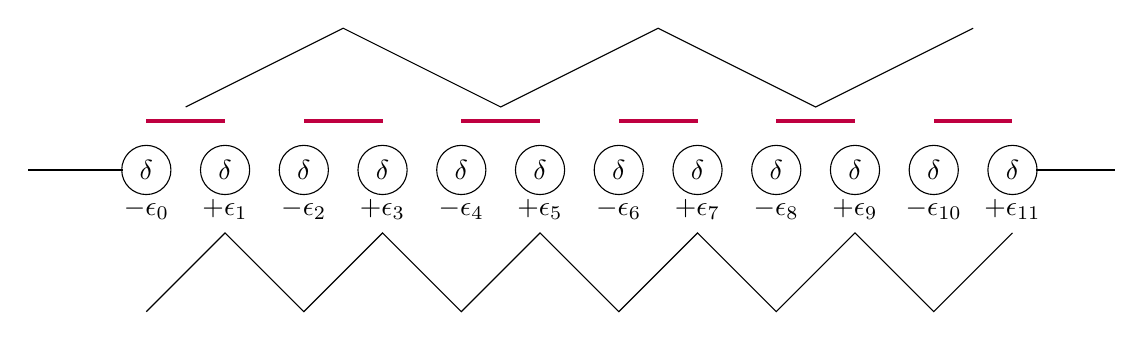
\begin{tikzpicture}

% Define coordinates for the zigzag pattern
\coordinate (A) at (1,0.3);
\coordinate (B) at (3,1.3);
\coordinate (C) at (5,0.3);
\coordinate (D) at (7,1.3);
\coordinate (E) at (9,0.3);
\coordinate (F) at (11,1.3);
%\coordinate (G) at (13,0);

% Draw the zigzag pattern
\draw (A) -- (B) -- (C) -- (D) -- (E) -- (F);

% Draw circles with text "4.3" inside
\foreach \x in {0.5, 1.5, 2.5, 3.5, 4.5,5.5,6.5,7.5, 8.5, 9.5, 10.5, 11.5} {
    \node[circle, draw, minimum size=.5cm] at (\x, -0.5) {$\delta$};
}

\coordinate (A) at (-1.0,-.5);
\coordinate (B) at (.2,-.5);
\draw (A) -- (B);

\coordinate (A) at (11.8,-.5);
\coordinate (B) at (12.8,-.5);
\draw (A) -- (B);

% Define coordinates for the zigzag pattern
\coordinate (A) at (0.5,-2.3);
\coordinate (B) at (1.5,-1.3);
\coordinate (C) at (2.5,-2.3);
\coordinate (D) at (3.5,-1.3);
\coordinate (E) at (4.5,-2.3);
\coordinate (F) at (5.5,-1.3);
\coordinate (G) at (6.5,-2.3);
\coordinate (H) at (7.5,-1.3);
\coordinate (I) at (8.5,-2.3);
\coordinate (J) at (9.5,-1.3);
\coordinate (K) at (10.5,-2.3);
\coordinate (L) at (11.5,-1.3);
% Draw the zigzag pattern
\draw (A) -- (B) -- (C) -- (D) -- (E) -- (F) -- (G) -- (H) -- (I) -- (J) -- (K) -- (L);

% Draw purple rectangles above the circles
\foreach \x in {0.5, 1.0} {
    \fill[purple] (\x-0.0, 0.1) rectangle (\x+.5, 0.15);
}

\foreach \x in {2.5, 3.0} {
    \fill[purple] (\x-0.0, 0.1) rectangle (\x+.5, 0.15);
}

\foreach \x in {4.5, 5.0} {
    \fill[purple] (\x-0.0, 0.1) rectangle (\x+.5, 0.15);
}

\foreach \x in {6.5, 7} {
    \fill[purple] (\x-0.0, 0.1) rectangle (\x+.5, 0.15);
}

\foreach \x in {8.5, 9} {
    \fill[purple] (\x-0.0, 0.1) rectangle (\x+.5, 0.15);
}

\foreach \x in {10.5, 11} {
    \fill[purple] (\x-0.0, 0.1) rectangle (\x+.5, 0.15);
}


% Add small annotations and text values
\node at (0.5, -1.) {$-\epsilon_0$};
\node at (1.5, -1.) {$+\epsilon_{1}$};
\node at (2.5, -1.) {$-\epsilon_{2}$};
\node at (3.5, -1.) {$+\epsilon_{3}$};
\node at (4.5, -1.) {$-\epsilon_{4}$};
\node at (5.5, -1.) {$+\epsilon_{5}$};
\node at (6.5, -1.) {$-\epsilon_{6}$};
\node at (7.5, -1.) {$+\epsilon_{7}$};
\node at (8.5, -1.) {$-\epsilon_{8}$};
\node at (9.5, -1.) {$+\epsilon_{9}$};
\node at (10.5, -1.) {$-\epsilon_{10}$};
\node at (11.5, -1.) {$+\epsilon_{11}$};




\end{tikzpicture}
   \caption{A tree with alternating weight assignment.}
    \label{fig:tree}
\end{figure}
    
    
    Now, consider the assignment (except for $\tilde{w}_i$ and $\tilde{w}_{4j+i}$): $\forall k,j$ 
    \begin{gather*}
        \epsilon_{4k+1} = \epsilon_0 + .2 + 10^{-k}\\
        \epsilon_{4k+3} = \epsilon_0 + 10^{-k}\\
        \epsilon_{2j} = \epsilon_0 
    \end{gather*}
    As argued above this assignment ensures strict comparisons (inequalities). Now, let
    \begin{align*}
        \tilde{w}_i, \tilde{w}_{4j+i} = \epsilon_0 + .1 + 10^{-\frac{i}{4}}.
    \end{align*}
    This forces the weighting $\tilde{w}$ to satisfy the comparison $(v_{2j + i}, v_{4j + i}, v_{i})$. We need to argue that all the other comparisons are satisfied according to the scheme above (\eqnref{eq: mod1}-\eqref{eq: mod4}).

    Now, consider the following assignment for $\hat{w}$:

\begin{equation}
    \hat{w}_l =\begin{cases}
        \epsilon_0 + .1 + 10^{-k} & \textnormal{ if } l = 4k+1 \ge 4j+i \textnormal{ or } l = 4k+3 \le i\\
        \epsilon_0 + .2 + 10^{-k} & \textnormal{ if } l = 4k+1 \le i\\
        \epsilon_0 + 10^{-k} & \textnormal{ if } l = 4k+3 \ge 4j+i\\
        \epsilon_0& \textnormal{ if } l = 2k\\
    \end{cases}
\end{equation}

It is easy to check that the assigned weighting $\hat{w}$ satisfies all the inequalities in \eqnref{eq: mod1}-\eqref{eq: mod4}. But then the learner maintains both the weightings $\hat{w}$ and $\tilde{w}$ in the version space $\sf{VS}(\cT)$. Thus, if the comparison $(v_{2j + i}, v_{i}, v_{4j + i})$ is not provided by the teacher, the learner maintains tree metrics not related up to triplet constraints. This contradicts the validity of the oblivious teaching set $\cT$ for \algoref{alg: tree}. Hence, there doesn't exist an oblivious teaching set for the weighting $\boldsymbol{w}$ on the path tree $G_{p}$ of size $O(n^2)$.
\end{proof}
\end{comment}

In \propref{prop: treelower}, we showed a lower bound on the size of triplet comparisons for \algoref{alg: tree}. Now, we show that the worst-case oblivious teaching complexity is tight.


\begin{proposition}
        For the distance model $\fin$ on a set $\cX$ of size $N$, the teaching complexity for \algoref{alg: tree} is $N(N-2)$ for oblivious teaching up to triplet equivalence. 
\end{proposition}
\begin{proof}
    Let $d_{w^*} \in \fin$ be an arbitrary target distance function for oblivious teaching in \algoref{alg: tree}. We show a construction of a teaching set $\cT(d_{w^*}, \fin)$ of size $N(N-2)$.
    The set is composed of the following set of triplet comparisons: 
    \begin{enumerate}
        %\item $T_{\sf{pos}} = \curlybracket{(x,y,z) \,|\, e_{xy},e_{xz} \in E(G^*), d_{w^*}(x,y) \ge d_{w^*}(x,z)}$
        %\item $T_{\sf{comp}} = \bigcup_{v \in \cX} \bigcup_{P \in T_v} \bigcup_{u \in P} \bigcup_{(P' \in T_v\setminus P)} \curlybracket{(u,v,y), (u,v,z)\,|\, \not\exists\, x' \neq y,z \in P' \textnormal{ s.t. } d_{w^*}(v,y) < d_{w^*}(v,x') < d_{w^*}(v,z) } $ where $T_v$ denotes a tree rooted at the node $v$ and $P$ denotes a subtree of $T_v \setminus \{v\}$.
        \item  $T_{\sf{comp}} = \bigcup_{v \in \cX} \curlybracket{(v, x, y)_{\ell}\,|\,  d_{w^*}(v,x) \ge d_{w^*}(v,y), \not\exists z \in \cX,\, d_{w^*}(v,x) > d_{w^*}(v,z)\textnormal{ or }d_{w^*}(v,z) > d_{w^*}(v,y)}$
    \end{enumerate}
    The key idea is to fix a pivot (a center node) and teach all the distances wrt that node in the finite sample space $\cX$. This is exactly what the comparisons in $T_{\sf{comp}}$ specify. Since any triplet comparison is centered this set sufficiently teaches the distance function $d_{w^*}$ on $\cX$.
 %   We can interpret $T_{\sf{pos}}$ as the set of comparisons for each node and adjacent edges. We can show that this set is sufficient to retain the tree structure $G^*$ of the target metric with the exact node connectivity, i.e. for all distinct metrics $(G', w'), (G'', w'') \in \sf{\cXS}(T_{\sf{pos}})$ we have $G' \cong G''$. 
    
    %The proof follows from two straight-forward observations: i) if $u$ is on the path in $G^*$ connecting $x,y \in \cX$ and (wlog) $d_{w^*}(u,x) \ge d_{w^*}(u,y)$, then the triplets $(u,x,y)$ and $(y, x, u)$ sufficiently specify that, and ii) if $e_{uv} \in E(G^*)$ for vertices $u,v\in \cX$ then there is no other path from $u$ to $v$ containing non-trivial vertex $x \in \cX$. With a simple manipulation, it is clear that the first one holds trivially. The second observation follows from a standard property of a tree graph where two nodes have a unique path connecting them. The rest of the proof uses these observations to drive an induction argument on the number of vertices. For the case when $|\cX| = 3$, the proof statement holds trivially. Now, assume it holds up to $|\cX| = k-1$. For the case $|\cX| = k$, consider a leaf node $v$ and all the triplets in $T_{\sf{pos}}$ that compares other nodes to $v$, call it $\cT_v$. Excluding these triplets induction argument and observation i) implies $G^*\setminus \{v\}$ is correctly identified. Now, if $v$ is connected to $u$ in $G^*$ then all the triplets in $\cT_v$ is wrt $u$. So, there doesn't exist a tree in which $v$ is connected to some $u' \neq u \in \cX$ otherwise there exists $x$ such that (wlog) $(u,v,x) \in \cT_v$ and is on the path connecting $u$ and $v$. But this contradicts the assumption that $u$ is on the unique path connecting $x$ and $v$ as implied by the choice of $\cT_v$ as shown in the observation i). Thus, $T_{\sf{pos}}$ sufficiently retains the structure of the tree $G^*$. We can count the size of $T_{\sf{pos}}$ as follows:
    %\begin{align*}
    %    |T_{\sf{pos}}| = 2\sum_{v \in \cX} \binom{\deg^+(v)}{2} \le 2\binom{\sum_{v \in \cX} \deg^+(v)}{2} = 2\binom{2(n-1)}{2} = 2(n-1)(2n-3)
    %\end{align*}
    %where we have used the convexity of $\binom{t}{2}$ for $t > 0$.
    
    %$T_{\sf{comp}}$ is the set of triplet comparisons wrt each vertex $v \in \cX$; essentially capturing the ordering of the distances wrt $v$. In order words, order all the distances $\curlybracket{ \forall x\in \cX, w^*(v,x)}$ inducing a ranking $\sigma_v$ on $\cX \setminus \{v\}$, i.e. 
    %\begin{align*}
    %    w^*(v,\sigma_v(x)) \ge w^*(v,\sigma_v(y)) \Longleftrightarrow \sigma_v(x) \succeq \sigma_v(y)
    %\end{align*}
    %But teaching this ranking only requires $(n-2)$ triplet comparisons. Since there are $n$ vertices, we need at the most $(n-2)n$ triplet comparisons to specify the entire weighting $w^*$ on $G^*$ up to triplet constraints relation.

    %Adding the sizes of $T_{\sf{pos}}$ and $T_{\sf{comp}}$ gives the stated upper bound on the oblivious teaching set for \algoref{alg: tree}. 
\end{proof}

\subsection{Bounds for quadruple comparisons}

In this subsection, we study the oblivious teaching complexity with quadruple comparisons. First, we will show that with $\binom{N}{2} -1 $ quadruple comparisons, the teacher can specify any symmetric distance function $d_w$ up to ordinal equivalence.
\begin{figure}[h]
\centering
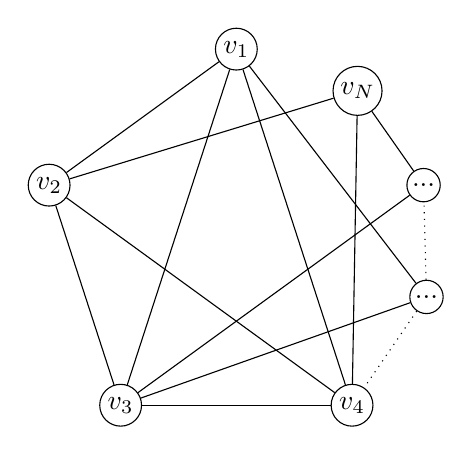
\begin{tikzpicture}
    % Parameters
    \def\radius{2.5cm} % Radius of the circle
    
    % Draw vertices in a circle and rename them
    \node[circle, draw, fill=white, inner sep=1.5pt] (v1) at (90:\radius) {$v_1$};
    \node[circle, draw, fill=white, inner sep=1.5pt] (v2) at (162:\radius) {$v_2$};
    \node[circle, draw, fill=white, inner sep=1.5pt] (v3) at (234:\radius) {$v_3$};
    \node[circle, draw, fill=white, inner sep=1.5pt] (v4) at (306:\radius) {$v_4$};
    \node[circle, draw, fill=white, inner sep=1.5pt] (vN_1) at (18:\radius) {$...$};
    \node[circle, draw, fill=white, inner sep=1.5pt] (vN_2) at (345:\radius) {$...$};
    \node[circle, draw, fill=white, inner sep=1.5pt] (v_N) at (52:\radius) {$v_N$};

    % Draw edges (adjust as needed)
    \draw (v1) -- (v2);
    \draw (v1) -- (v3);
    \draw (v2) -- (v3);
    \draw (v2) -- (v4);
    \draw (v3) -- (v4);

    \draw (v1) -- (v4);
    \draw (v_N) -- (v4);
    \draw (v_N) -- (v2);
    \draw (vN_2) -- (v3);
    \draw (vN_1) -- (v3);
    \draw (vN_2) -- (v1);
    \draw[dotted] (vN_2) -- (vN_1);
    \draw[dotted] (vN_2) -- (v4);
    \draw (v_N) -- (vN_1);
\end{tikzpicture}
\caption{A finite sample distance function}
        \label{fig:graph_metric}
\end{figure}
\begin{proposition} 
Consider a symmetric distance function $d_w$ on a finite sample $\cX$ of size $N$. With $\binom{N}{2} - 1$ many quadruple comparisons an oblivious learner can exactly learn $d_w$ up to ordinal equivalence.
\end{proposition}
\begin{proof}
    We can order the weight $w: \cX \times \cX \to \reals_{+}$ over any pair of vertices in $\cX$ as
    \begin{align}
        w_1 \le w_2 \le w_3 \le \ldots \le w_{\binom{N}{2}}   \label{eq: ordering}
    \end{align}
    (there are $\binom{N}{2}$ many pairs). Thus, if we provide the quadruple comparisons for each $i$ $w_i \le w_{i+1}$, i.e $(u_i, v_i , u_{i+1}, v_{i+1})_{\ell}$ where $(u_i, v_i)$ is the vertices pair for the distance $w_i$, similarly $(u_{i+1}, v_{i+1})$ for $w_{i+1}$. Thus, the set of quadruplets:
    \begin{align*}
        Q = \curlybracket{(u_i, v_i , u_{i+1}, v_{i+1})_{\ell} \,|\, i \in [n-1],\, d_w(u_i, v_i) = w_i}
    \end{align*}
    Note that $|Q| = \binom{N}{2} - 1$. $Q$ exactly specifies the ordering over all the distances, thus if the learner learns a distance function $d_{w'}$ over $\cX$ then the weights corresponding to the same pair of vertices in maintain the ordering of \eqnref{eq: ordering}. This implies that no matter the weights $w'$ assigned by the learner they are ordinally equivalent to $w$. Hence, the claim of the proposition is proven.
\end{proof}

\begin{figure}[h]
\centering
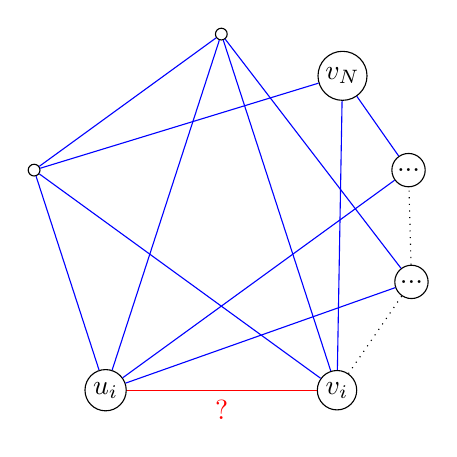
\begin{tikzpicture}
    % Parameters
    \def\radius{2.5cm} % Radius of the circle
    
    % Draw vertices in a circle and rename them
    \node[circle, draw, fill=white, inner sep=1.5pt] (v1) at (90:\radius) {};
    \node[circle, draw, fill=white, inner sep=1.5pt] (v2) at (162:\radius) {};
    \node[circle, draw, fill=white, inner sep=1.5pt] (v3) at (234:\radius) {$u_i$};
    \node[circle, draw, fill=white, inner sep=1.5pt] (v4) at (306:\radius) {$v_i$};
    \node[circle, draw, fill=white, inner sep=1.5pt] (vN_1) at (18:\radius) {$...$};
    \node[circle, draw, fill=white, inner sep=1.5pt] (vN_2) at (345:\radius) {$...$};
    \node[circle, draw, fill=white, inner sep=1.5pt] (v_N) at (52:\radius) {$v_N$};

    % Draw edges (adjust as needed)
    \draw[blue] (v1) -- (v2);
    \draw[blue] (v1) -- (v3);
    \draw[blue] (v2) -- (v3);
    \draw[blue] (v2) -- (v4);
    \draw[red] (v3) -- (v4) node[midway, below] {?};

    \draw[blue] (v1) -- (v4);
    \draw[blue] (v_N) -- (v4);
    \draw[blue] (v_N) -- (v2);
    \draw[blue] (vN_2) -- (v3);
    \draw[blue] (vN_1) -- (v3);
    \draw[blue] (vN_2) -- (v1);
    \draw[dotted] (vN_2) -- (vN_1);
    \draw[dotted] (vN_2) -- (v4);
    \draw[blue] (v_N) -- (vN_1);
\end{tikzpicture}
\caption{A finite sample distance function}
        \label{fig:counter_metric}
\end{figure}
Now, we will also provide a tight lower bound on the quadruple comparisons via showing a lower bound on oblivious teaching complexity for a finite-sample distance function, where we further assume that it satisfies the triangle inequality.

%\begin{lemma}
%    There exists a graph distance function $(G, d_G)$ such that the teacher needs to necessarily provide $\binom{n}{2} - 1$ quadruple comparisons in order for the learner to identify the target graph distance function. 
%\end{lemma}
%\begin{proof}
%    For the sake of contradiction, assume the contrary on the worst-case lower bound.   We will construct a counterexample based on a graph metric of size $n > 2$. We will show an assignment of weight $W_G$ which can't be taught in fewer than $\binom{n}{2} - 1$ many quadruple comparisons.

%    Lets fix a large positive scalar $\hat{w} > 0$ (sufficient choice would be clear from the discussion). Now, consider a weighting $W_G$ where for any $v_k, v_m \in G$, $d(v_k, v_m) = \hat{w} + \epsilon_{km}$ where $\epsilon_{km} > 0$. Assume that $\epsilon_{km}$ is within $(\epsilon, 2\epsilon)$ where $\epsilon > 0 $ is comparatively smaller than $\hat{w}$. 
%    Now, note that for any vertices $v_a, v_b,v_c \in \cX$, we obtain lower bounds and upper bounds on the distances within these vertices using the triangle inequality property of the metric $d$, i.e.
%    \begin{align*}
%        d(v_a, v_b) + d(v_b, v_c) \ge d(v_a, v_c) \ge |d(v_a, v_b) - d(v_b, v_c)|
%    \end{align*}
%    Thus, $d(v_a, v_c)$ can attain any value that satisfies these inequality and the distance function induced by these three vertices is a valid metric (other properties are trivially satisfied). We will use his observation to show that teacher needs to provide quadruple comparisons with respect to any pair $(v_i, v_j) \in G$.
%    Now, consider an ordering of weights in $W_G$ as shown in \eqnref{eq: ordering}. WLOG assume that for a weight $w_i$ corresponding to vertices $u_i$ and $v_i$ is not specified correctly in the ordering, i.e. for
%    \begin{align*}
%        w_{i-1} \le w_i \le w_{i+1}
%    \end{align*}
%    at least one of the quadruple comparisons---$(u_{i-1},v_{i-1},u_{i},v_{i})$ or $(u_{i},v_{i},u_{i+1},v_{i+1})$ are not provided by the teacher. Assume it is $(u_{i-1},v_{i-1},u_{i},v_{i})$. We can show that even if all the other quadruple comparisons are provided an oblivious learner can't find the exact ordering of $w_i$ wrt $w_{i-1}$. In fact, learner maintains a weight $w'_G$ in which $d'(u_i,v_i) < d'(u_{i-1},v_{i-1})$ but all the other quadruple comparisons are satisfied.

%    Fixing $u_i$ and $v_i$, consider all the possible triangle inequalities for any vertex $v \in \cX \setminus \{u_i,v_i\}$. Due to the choice of the target weighting $w_G$, $d(u_i,v_i)$ has to satisfy the following inequalities to be consistent with every distance corresponding to the vertex $v$:
%    \begin{align}
%        2 \epsilon \le d(u_i,v_i) \le 2\hat{w} + \epsilon \label{eq1}
%    \end{align}
%    But then,
%    \begin{align*}
%       \hat{w} + \epsilon \le  w_{i-1} = d(u_i,v_i) \le \hat{w} + 2\epsilon
%    \end{align*}
%    Since $\epsilon$ is comparatively smaller than $\hat{w}$, 
%    \begin{align}
%        2 \epsilon < w_{i-1} < 2\hat{w} + \epsilon \label{eq2}
%    \end{align}
%    Thus, using \eqnref{eq1} and \eqnref{eq2} the learner can pick/assign a weight for $d'(u_i,v_i)$ either in the interval $(2\epsilon, w_{i-1})$ or $(w_{i-1}, 2\hat{w} + \epsilon)$ and still satisfy all the quadruple comparisons given by the teacher for they are consistent with \eqnref{eq: ordering}. Hence, the teacher has to provide the comparison $(u_{i-1},v_{i-1},u_{i},v_{i})$. Similarly one can argue for the case when the teacher omits the comparison $(u_{i},v_{i},u_{i+1},v_{i+1})$. This completes the proof of the stated claim and thus we achieve a lower bound of $\binom{n}{2} -1$ on the number of quadruple comparisons for oblivious teaching.
%\end{proof}


\begin{lemma}
    For any symmetric distance function $d_w$ on the finite sample space $\cX$ the teacher needs to necessarily provide $\binom{N}{2} - 1$ quadruple comparisons for the learner to identify the target distance function up to ordinal equivalence. 
\end{lemma}

\begin{proof}
    For any symmetric distance function $d_w$, note that there are $\binom{N}{2}$ distances corresponding to any pair $\curlybracket{x,y}$ of vertices in $\cX$. Consider the ordering $\sigma_w$ of the weights:
    \begin{align*}
        w_1 \le w_2 \le \ldots \le w_{\binom{N}{2}}
    \end{align*}
    where each $w_i$ corresponds to a unique pair of vertices in $\cX$. A distance function $d_{w'}$ is ordinally equivalent to $d_w$ only if $w'$ assigns the same ordering $\sigma_{w'} = \sigma_w$ over the pairs of vertices. 

    WLOG assume that for a weight $w_i$ corresponding to vertices $u_i$ and $v_i$ is not specified correctly in the ordering, i.e. for
    \begin{align*}
        w_{i-1} \le w_i \le w_{i+1}
    \end{align*}
    at least one of the quadruple comparisons---$(u_{i-1},v_{i-1},u_{i},v_{i})_{\ell}$ or $(u_{i},v_{i},u_{i+1},v_{i+1})_{\ell}$ are not provided by the teacher. Assume it is $(u_{i-1},v_{i-1},u_{i},v_{i})_{\ell}$. We can show that even if all the other quadruple comparisons are provided an oblivious learner can't find the exact ordering of $w_i$ wrt $w_{i-1}$. In fact, learner maintains a weight $w'$ in which $d_{w'}(u_i,v_i) < d_{w'}(u_{i-1},v_{i-1})$ but all the other quadruple comparisons are satisfied. Since $w'_i$ is only required to be a positive scalar, the learner can maintain any ordering of $w'_i$ by assigning a value smaller than $w'_{i-1}$ inducing a different ordering than $\sigma_w$. A contradiction. 

    Hence, the teacher has to provide the comparison $(u_{i-1},v_{i-1},u_{i},v_{i})_{\ell}$. Similarly one can argue for the case when the teacher omits the comparison $(u_{i},v_{i},u_{i+1},v_{i+1})_{\ell}$ (assuming $w_i$ is not the largest weight in the ordering). This completes the proof of the stated claim and thus we achieve a lower bound of $\binom{N}{2} -1$ on the number of quadruple comparisons for oblivious teaching.

    
    %Fixing $u_i$ and $v_i$, consider all the possible triangle inequalities for any vertex $v \in \cX \setminus \{u_i,v_i\}$. Due to the choice of the target weighting $w_G$, $d(u_i,v_i)$ has to satisfy the following inequalities to be consistent with every distance corresponding to the vertex $v$:
    %\begin{align}
    %    2 \epsilon \le d(u_i,v_i) \le 2\hat{w} + \epsilon \label{eq1}
    %\end{align}
    %But then,
    %\begin{align*}
    %   \hat{w} + \epsilon \le  w_{i-1} = d(u_i,v_i) \le \hat{w} + 2\epsilon
    %\end{align*}
    %Since $\epsilon$ is comparatively smaller than $\hat{w}$, 
    %\begin{align}
    %    2 \epsilon < w_{i-1} < 2\hat{w} + \epsilon \label{eq2}
    %\end{align}
    %Thus, using \eqnref{eq1} and \eqnref{eq2} the learner can pick/assign a weight for $d'(u_i,v_i)$ either in the interval $(2\epsilon, w_{i-1})$ or $(w_{i-1}, 2\hat{w} + \epsilon)$ and still satisfy all the quadruple comparisons given by the teacher for they are consistent with \eqnref{eq: ordering}. Hence, the teacher has to provide the comparison $(u_{i-1},v_{i-1},u_{i},v_{i})$. Similarly one can argue for the case when the teacher omits the comparison $(u_{i},v_{i},u_{i+1},v_{i+1})$. This completes the proof of the stated claim and thus we achieve a lower bound of $\binom{n}{2} -1$ on the number of quadruple comparisons for oblivious teaching.
    
    
\end{proof}

\newpage
%\paragraph{Sampled triplet comparisons for a graph metric:} We can study the notion of oblivious teaching of a tree metric for a sampled triplet comparison from the set $\curlybracket{(u,x,y)\,|\, u,x,y \in G}$. We can study the teaching complexity for $\epsilon$-accuracy as in \defref{defn: lebsample} under a discrete distribution over the triplets. Denote the set of all possible triplet as $\cT_{\sf{all}}$ for a vertex set $\cX$ and metric model $\tree$.
%\begin{lemma}
%    Consider a distribution $\cD$ over $\cT_{\sf{all}}$. For any $\epsilon \in (0,1]$, the worst-case oblivious teaching complexity for \algoref{alg: tree} has a lower bound of $\Omega\paren{n^2}$ that achieves $\epsilon$-accuracy for teaching up to triplet constraints relation $\sim_{tree}$. Furthermore, the lower bound for $1$-accuracy is $\Omega\paren{n^3}$.
%\end{lemma}
%\begin{proof}
%    This is a straight-forward implication of the construction in \propref{prop: treelower}. 
%\end{proof}
%\begin{lemma}
%    Consider a distribution $\cD$ over $\cT_{\sf{all}}$. For any $\epsilon \in (0,1]$, the worst-case oblivious teaching complexity for \algoref{alg: tree} has a lower bound of $\Omega\paren{n^2}$ that achieves $\epsilon$-accuracy for teaching up to triplet constraints relation $\sim_{tree}$. Furthermore, the lower bound for $1$-accuracy is $\Omega\paren{n^3}$.
%\end{lemma}




